
%% bare_conf.tex
%% V1.3
%% 2007/01/11
%% by Michael Shell
%% See:
%% http://www.michaelshell.org/
%% for current contact information.
%%
%% Support sites:
%% http://www.michaelshell.org/tex/ieeetran/
%% http://www.ctan.org/tex-archive/macros/latex/contrib/IEEEtran/
%% and
%% http://www.ieee.org/

%%*************************************************************************
%% Legal Notice:
%% This code is offered as-is without any warranty either expressed or
%% implied; without even the implied warranty of MERCHANTABILITY or
%% FITNESS FOR A PARTICULAR PURPOSE!
%% User assumes all risk.
%% In no event shall IEEE or any contributor to this code be liable for
%% any damages or losses, including, but not limited to, incidental,
%% consequential, or any other damages, resulting from the use or misuse
%% of any information contained here.
%%
%% All comments are the opinions of their respective authors and are not
%% necessarily endorsed by the IEEE.
%%
%% This work is distributed under the LaTeX Project Public License (LPPL)
%% ( http://www.latex-project.org/ ) version 1.3, and may be freely used,
%% distributed and modified. A copy of the LPPL, version 1.3, is included
%% in the base LaTeX documentation of all distributions of LaTeX released
%% 2003/12/01 or later.
%% Retain all contribution notices and credits.
%% ** Modified files should be clearly indicated as such, including  **
%% ** renaming them and changing author support contact information. **
%%
%% File list of work: IEEEtran.cls, IEEEtran_HOWTO.pdf, bare_adv.tex,
%%                    bare_conf.tex, bare_jrnl.tex, bare_jrnl_compsoc.tex
%%*************************************************************************

%
\documentclass[conference]{IEEEtran}
\usepackage{cite}
\ifCLASSINFOpdf
  \usepackage[pdftex]{graphicx}
\fi
\usepackage[cmex10]{amsmath}
\usepackage{algorithmic}
\usepackage{array}
\usepackage{fixltx2e}
\usepackage{url}

% added
\usepackage{amssymb}
\usepackage[ruled,vlined]{algorithm2e}
\usepackage{stmaryrd}


\newtheorem{property}{Property}
\newtheorem{assumption}{Assumption}
\newtheorem{theorem}{Theorem}
\newtheorem{definition}{Definition}
\newtheorem{lemma}{Lemma}
\newtheorem{remark}{Remark}
\newtheorem{constraint}{Constraint}
\newtheorem{corollary}{Corollary}
\newtheorem{condition}{Condition}

\def\QED{\mbox{\rule[0pt]{1.5ex}{1.5ex}}}
\def\proof{\noindent{{\textbf{Proof}: }}}
\def\endproof{\hspace*{\fill}~\QED\par\endtrivlist\unskip \vspace{1\baselineskip}}

\newcommand{\dbf}[1]{\operatorname{dbf}(#1)}

\algsetup{
  indent=1em,
  linenosize=\small,
  linenodelimiter=\
}

% correct bad hyphenation here
\hyphenation{op-tical net-works semi-conduc-tor}


\begin{document}
\title{The Space of Feasible Execution Times for Asynchronous Periodic Task
Systems using Definitive Idle Times}


\author{
\IEEEauthorblockN{Thomas Chapeaux and Paul Rodriguez}
\IEEEauthorblockA{Universit\'{e} Libre de Bruxelles / ECE Paris\\
tchapeau@ulb.ac.be, paurodri@ulb.ac.be}
\and
\IEEEauthorblockN{Laurent George}
\IEEEauthorblockA{University of Paris-Est / ECE Paris\\
lgeorge@ieee.org}
\and
\IEEEauthorblockN{Jo\"el Goossens}
\IEEEauthorblockA{Universit\'{e} Libre de Bruxelles\\
joel.goossens@ulb.ac.be}
}

\maketitle

\begin{abstract}
	Sensitivity analysis for real-time systems provides efficient methods to determine feasibility
	conditions in the case of changes in task parameters, such as
	different WCET values when porting a system to a different platform. The \mbox{C-space} defines the space of execution
	times for which a system is feasible, which can help system designers to more easily check
	if a task set is feasible on a set of candidate platforms. This paper extends previous works
	generalizing the description of the C-space for Earliest Deadline First
	scheduling to systems with initial task offsets. The feasibility gain offered
	by offsets is then expressed as the volume ratio between the C-space of an
	asynchronous system and its corresponding synchronous system when offsets are randomly chosen. The problem
	requires solving multiple similar instances of the Chinese Remainder Problem,
	for which an efficient algorithm in this context is provided. We show that even for random offsets, the gain can reach 15\%.
\end{abstract}

% For peer review papers, you can put extra information on the cover
% page as needed:
% \ifCLASSOPTIONpeerreview
% \begin{center} \bfseries EDICS Category: 3-BBND \end{center}
% \fi
%
% For peerreview papers, this IEEEtran command inserts a page break and
% creates the second title. It will be ignored for other modes.
%\IEEEpeerreviewmaketitle

\section{Introduction}

	Abstract models for real-time systems often require the determination of the
	worst-case execution time of a job (WCET), a value highly dependent on the
	platform on which the application is deployed. Feasibility conditions allow us to
	decide whether a system can be correctly scheduled (i.e. without violating any
	timeliness constraint) based on task parameters, including the WCET.

	The \mbox{C-space} of a real-time system is, intuitively,
	the space of WCET values for which this system is feasible
	\cite{bini2004schedulability,george2009characterization}. A precise and efficient description of the C-space of a system would allow us to efficiently decide whether or not it is feasible on a set of candidate platforms.

	In section~\ref{sct:relatedWorks}, the description of the C-space of synchronous
	constrained systems, which has been mostly covered by \cite{george2009characterization}, is revisited.
	This description is based on the Demand Bound Function (DBF) feasibility condition described in
	\cite{baruah1999generalized,baruah1990algorithms} and is found with exponential complexity using
	the notion of definitive idle times (DIT). The DIT notion provides a feasibility interval for EDF that does not depend of the WCET of the tasks.

	In section~\ref{sct:asyncDIT}, we present an extension of the concept of DIT adapted to the
	asynchronous case called first periodic DIT
	($t_d$) along with an algorithm to determine its existence and value for any system,
	then we show the influence of some factors on its existence.

	In Section~\ref{sct:asyncCspace}, we show how to describe the C-space of an asynchronous
	system based on the demand bound function test. Then we show why applying this
	test on the interval starting at $t_d$
	and spanning an hyperperiod is sufficient when $t_d$ exists. A
	numerical example is also given.

	Finally, in section~\ref{sct:expCspaceGain}, we use a simulation to quantify the feasibility
	gain of asynchronous systems in terms of volume of the C-space.

\section{Related works}
\label{sct:relatedWorks}

%Review 3 : add map of literature

	\subsection{Model}
		We consider a discrete timeline and tasks systems comprised of periodic
		tasks with constrained deadlines on uniprocessor platforms. Each task
		$\tau_i$ is represented by a tuple $(O_i, C_i, D_i, T_i)$ where $O_i$ is the offset value,
		$C_i$ the WCET, $D_i$ the relative deadline and $T_i$ the period, which is the exact time between two consecutive arrivals.
		The constrained deadline property implies that $D_i \leq T_i$. In
		the following, we differentiate between \emph{synchronous systems} (where $O_i
		= 0$ for all tasks) and \emph{asynchronous systems} (which are not synchronous).

		For both synchronous and asynchronous systems, the preemptive
		\emph{Earliest Deadline First} (EDF) algorithm, in which jobs are prioritized according to their absolute deadline, has been
		shown to be optimal \cite{liu1973scheduling}, which means it
		correctly schedules any feasible system within that group.

		Furthermore, we define:
		\begin{itemize}
			\item $\tau = \{\tau_1, \cdots, \tau_{n}\}$ is called the task system
			\item $H = \operatorname{lcm}(T_1, \cdots, T_{n})$
			\item $O_{max} = \max (O_1, \cdots, O_{n})$
			\item An \emph{idle time} is an instant $t$ at which each job that arrived
			strictly before $t$ has finished its execution.
			\item A \emph{busy period} is a time interval between two consecutive idle times in
			which at least one job is executing.
			\item The interval between the initial time ($t=0$) and the first
			idle time after $t=0$ is called the \emph{first busy period}.
		\end{itemize}

	\subsection{The DBF feasibility test}
		We recall the necessary and sufficient feasability condition on uniprocessor
		platforms based on the demand-bound function \cite{baruah1999generalized,
		baruah1990algorithms}.

		\begin{definition}
			The \textbf{demand-bound function (DBF)}
			defined for a task set $\tau$ in a time interval $[t_1, t_2]$ and denoted $\dbf{t_1, t_2}$, is
			equal to the cumulated execution time of jobs of $\tau$ contained in the
			closed interval $[t_1, t_2]$.
		\end{definition}

		Mathematically,
		\begin{equation}
			\dbf{t_1, t_2} = \sum_{i=1}^{n} n_i(t_1, t_2) \, C_i
		\end{equation}
		where $n_i(t_1, t_2)$ is the number of jobs of task $\tau_i$ which arrival times
		and deadlines are both in the closed interval $[t_1, t_2]$.

		The values of the $n_i$ are given by \cite{baruah1990algorithms}
		\begin{equation}
			n_i(t_1, t_2) =
			\left\llbracket
				\left\lfloor
					\frac{t_2 - O_i - D_i}{T_i}
				\right\rfloor -
				\left\lceil
					\frac{t_1 - O_i}{T_i}
				\right\rceil + 1
			\right\rrbracket_0
		\end{equation}
		where $\llbracket x \rrbracket_0$ stands for $\max \{ 0, x \}$.

		The following theorem is a necessary and sufficient condition of feasibility
		based on the DBF, given in \cite{baruah1999generalized}:
		\begin{theorem}
			\begin{equation*}
				\begin{array}{c}
					\tau \: \text{is feasible}  \iff
					\dbf{t_1, t_2} \leqslant t_2 - t_1 \; \forall t_1, t_2 \mid  0 \leq t_1 \leq t_2
				\end{array}
			\end{equation*}
		\end{theorem}
        %It is easy to see that the condition is at least necessary, as if there exists values of $t_1$ and $t_2$ such that $\dbf{t_1, t_2} > t_2 - t_1$, it means that more than $t_2 - t_1$ units of computation have to be done in $t_2 - t_1$ units of time. Therefore the system would not be feasible.

	\subsection{C-space of synchronous systems}
	\label{sct:cspaceDescr}

			The authors of \cite{george2009characterization} give the following definition of the C-space (based on \cite{bini2004schedulability}):
			\begin{definition}
				The \textbf{C-space} of a task system $\tau$ is a region of $n$ dimensions (where each dimension denotes the possible $C_i$ of a task of $\tau$) such that for any vector $C = \{ C_1, \cdots, C_{n}\}$ in it, $\tau$ is feasible.
			\end{definition}

			As explained in \cite{nemhauser1988integer}, a region of $\mathbb{N}_0^n$
			such as the C-space can be described by a \emph{polytope}, or a list of
			parametric linear constraints (called the \emph{formulation}). The
			constraints must be conditions which can unequivocally decide if a point is
			included in the region or not. In the sequel we give a formulation for the
			C-space in $\mathbb{N}_0^n$ (For a formulation in $\mathbb{N}^n$, we can add
			$C_i \geqslant 1 \; \forall \tau_i \in \tau$ to the list of constraints).

		The DBF test gives us the following list of inequations on the WCET values of the task set
		which, taken together, are a necessary and sufficient condition of feasibility:
		\begin{equation}
			\sum_{i=1}^{n}  n_i(t_1, t_2) \cdot C_i \leq t_2 - t_1 \; \forall t_1,t_2 \mid 0 \leq t_1 \leq t_2
		\end{equation}
		Note that for given values  of $(t_1, t_2)$, the $n_i(t_1, t_2)$ are
		constant (w.r.t. the $C_i$). Those inequations are thus indeed linear.

      However, this description contains an infinite number of constraints, most of
      which are redundant. While this does not harm the precision of the
      test, a finite description is needed in practice. The description should also be as small as possible as this can greatly
      reduce the computation time of practical feasibility tests. In Section~\ref{sct:removeRedundancy} a method to reduce the size of this set of constraints is given.

  \subsection{Removing redundant constraints}
    \label{sct:removeRedundancy}

  In the synchronous case, is has been shown in \cite{baruah1990algorithms} that the constraints corresponding
  to every interval $[0, t]$ (with $t$ a job deadline happening before $H$) are
  necessary and sufficient to test the feasibility of a system.

  Even then, the number of constraints to consider is exponential in the number
  of tasks. While it has been shown that constraints that cover intervals ending
  after the end of the first busy period are also redundant, this value depends on the $C_i$ and is
  therefore not usable for the purposes of this paper. The
  following concept, initially described by \cite{lipariaverage}, is thus introduced. It gives an upper bound for the end of the first busy period and does not depend on the execution times.

  \begin{definition}
    A \textbf{definitive idle time} (DIT) \cite{lipariaverage} is a time $t$ (if it exists) such that every job
    released strictly before instant $t$ has its absolute deadline before or at instant $t$.
  \end{definition}

  \begin{definition}
    The earliest DIT (if it exists) occurring in the system strictly after $t=0$ is called the
    \textbf{first DIT}, denoted $t_d$.
  \end{definition}

		\begin{remark} (from previous definitions):
			\begin{itemize}
				\item Contrary to other idle times, DITs are independent of the
					scheduling or the execution times of the jobs.
				\item In a feasible system, every DIT is an idle time.
				\item In a feasible system, the first DIT happens after the end of the
					first busy period if it exists.
				\item In synchronous systems any $kH$ with $k \geqslant 0$ is a DIT and we
					also have $t_d \leqslant H$.
			\end{itemize}
		\end{remark}

		% The value of the first DIT can be found by solving the following modular
		% equations system:
		% \begin{equation}
		% 	\begin{split}
		% 		 t_d = \min(& \{ t \; s.t. \; t > 0 \; and \\
		% 				& \forall \tau_i \in \tau, \; \exists a_i \in [D_i, T_i]: t \equiv a_i \;
		% 				(mod \; T_i) \})
		% 	\end{split}
		% \end{equation}
  The authors of \cite{george2009characterization} give a method to find the value of $t_d$ for cases in which periods are pairwise coprime.

  For synchronous systems in which the execution times are not known, the first DIT $t_d$
  is our ``best guess'' at an upper limit on the end of the busy period. As it was sufficient
  to check the DBF test in intervals $[0, t]$ before the end of the first busy period. This time interval is WCETs dependant. A more general feasility condition valid for any WCET is as follows:
  \begin{equation}
  		\dbf{0,t} \leqslant t \; \forall t \leqslant t_d
  		\iff \text{The system is feasible}
  \end{equation}

  To summarize, the description of the C-space is reduced from an infinite number
  of constraints to only those where $t_1 = 0$, $t_2 \leqslant t_d$ and
  values of $t_2$ correspond to job deadlines. Note that the number of
  constraints is still exponential in the number of tasks in the worst-case (which is when $t_d = H$).

\section{DIT in asynchronous systems}
  \label{sct:asyncDIT}

  \subsection{Definition}

    In an asynchronous system, the first DIT may happen before $O_{max}$, i.e. before all tasks are in the system. We thus introduce the following notion:

    \begin{definition}
      The \textbf{first periodic DIT} (FPDIT) of a system is the earliest DIT occurring
      strictly after $O_{max}$.
    \end{definition}

    By a slight abuse of notation, it will also be noted $t_d$. Note that in the
    synchronous case the first periodic DIT is also the first DIT.

	\subsection{Existence condition}
	\label{sct:FPDITexist}
		As in the synchronous case, the problem of existence of the FPDIT
		can be written as a system of modular equations:
		\begin{equation}
			\begin{array}{l}
				\exists ? \; t_d \; s.t. \; \forall \tau_i \in \tau, \exists a_i \in [D_i,
				T_i] \; :\\
				\left\{
					\begin{array}{l}
						t_d > O_i \\
						t_d - O_i \equiv a_i \; (mod \;	T_i)
						\\
					\end{array}
				\right.
			\end{array}
		\end{equation}
        Where $a \equiv b \; (mod \; n)$ means that $a$ and $b$ are congruent modulo $n$.

		This system is equivalent to multiple instances (one per combination of $a_i$
		values) of the Chinese Remainder Problem (CRP) where the goal is to find the
		value of $t_d$ such that it is congruent to $a_i+O_i$ modulo $T_i$ for all
		tasks $\tau_i$ in $\tau$. To find the FPDIT it is to the best of our knowledge
		necessary to solve the problem on all combinations of $a_i$ values and then
		to compute the minimum solution. We define $A_i = [D_i,T_i]$, $X_i = \{x_i
		= a_i+O_i \mid a_i \in A_i\}$ and $n_i = T_i$ for clarity in the context of
		the CRP.
		One instance of this problem is guaranteed to have at least one solution modulo $H$ for given values of $a_i$ if and only if
		Condition~\ref{eq:CRPcond} is satisfied \cite{knuth1969art}:
		\begin{equation}
			\label{eq:CRPcond}
			x_i \equiv x_j \; (\operatorname{mod} \; \operatorname{gcd}(n_i, n_j))
			\; \forall \tau_i,\tau_j \in \tau
		\end{equation}
		Condition~\ref{eq:CRPcond} means that DITs might still exist even though in
		the general case task periods will not necessarily be pairwise coprime.
% 		We now present an example of such a system.\\
%
% 		\begin{center}
% 			\begin{tabular}{|r|c|c|c|c|}
% 				\hline
% 							& $O_i$ & $C_i$ & $D_i$ & $T_i$ \\ \hline
% 				$\tau_1$ 	& 0 	& $C_1$ & 3 	& 4\\ \hline
% 				$\tau_2$ 	& 2 	& $C_2$ & 7 	& 8\\ \hline
% 			\end{tabular}
% 		\end{center}
%
% 		Here, the possible values of $a_1$ are 3 and 4, and the possible values
% 		of $a_2$ are 7 and 8. For a FPDIT to exist, one of the following
% 		conditions must be fulfilled:
% 		\[
% 			\left[
% 			\begin{array}{c}
% 				3 + 0 \equiv 7 + 2 \; (\operatorname{mod} \; 4 ) \\
% 				3 + 0 \equiv 8 + 2 \; (\operatorname{mod} \; 4 ) \\
% 				4 + 0 \equiv 7 + 2 \; (\operatorname{mod} \; 4 ) \\
% 				4 + 0 \equiv 8 + 2 \; (\operatorname{mod} \; 4 ) \\
% 			\end{array}
% 			\right.
% 		\]
% 		However neither is, which means the system has
% 		no FPDIT (and no other DIT than $t=0$).

	\subsection{Solving the modular system}
		A sketch of the construction algorithm to compute $t_d$ can be found in
		Algorithm~\ref{alg:algoCRP} (note that $x^{-1} \; (mod \; y)$ means the
		modular inverse of $x$ in the naturals modulo $y$). The congruences must
		first be modified in order to obtain pairwise coprime moduli. Each $n_i$
		is factored into prime powers $p^{k_1}_1 p^{k_2}_2 \cdots p^{k_m}_m = n_i$
		with $k_j$ the highest integer s.t. $p^{k_j}_j$ divides $n_i \; \forall j
		\; \mid 1 \leqslant j \leqslant m$. Each original constraint $t_d \equiv x_i
		\; (mod \; n_i)$ is replaced by the equivalent set
		\begin{equation*}
			\begin{split}
				t_d \equiv x_i 	& \; (mod \; p^{k_1}_1) \\
				t_d \equiv x_i 	& \; (mod \; p^{k_2}_2) \\
								& \vdots \\
				t_d \equiv x_i 	& \; (mod \; p^{k_m}_m) \\
			\end{split}
		\end{equation*}
		This operation (later called constraint \emph{factorisation}) might create
		duplicate constraints, which are removed.
		As shown in \cite{knuth1969art}, the resulting system can be solved using
		Algorithm~\ref{alg:algoCRP}. For ease of reading, we call $C$ the set of
		resulting constraints $c$ each written $t_d \equiv x_c \; (mod \;
		p_c)$.

		\begin{algorithm}
			\caption{Gauss's CRP Algorithm}
			\label{alg:algoCRP}
			\begin{algorithmic}[1]
				\REQUIRE $H$ is the hyperperiod of the system
				\FORALL{$c \in C$}
					\STATE $Mc \leftarrow \frac{H}{p_c}$
					\STATE $invMc \leftarrow Mc^{-1} \; (mod \; p_c)$
					\STATE $e_c \leftarrow Mc \cdot invMc$
				\ENDFOR
				\RETURN $\sum\limits_{c \in C}{x_c \cdot e_c} \; (mod \; H)$
			\end{algorithmic}
		\end{algorithm}


		%TODO change algo 2 with respect to explanation of coprime n_i

		Algorithm~\ref{alg:algoCRP} finds one DIT given one combination of $a_i$
		values. However using it in practice is very inefficient as there are
		exponentially many different combinations of $a_i$ values in the number of
		tasks (the cartesian product of all the $A_i$ sets), and resolving
		exponentially many CRP instances is prohibitively slow.
		A faster method for finding the FPDIT consists in merging all these CRP
		instances into one problem (finding all DITs), which can be solved faster by
		Algorithm~\ref{alg:multiACRP}, as a significant part of the intermediate
		results are shared between instances. The first part consisting in splitting
		all constraints into sets of constraints with prime power moduli is slightly
		different. We define for each task $\tau_i$ and $a_j \in A_i$ :
		$C_{ij}$ is the set of constraints resulting from the factorisation of $t_d
		\equiv a_j+O_i \; (mod \; n_i)$ of the form $t_d \equiv x_c
		\; (mod \; p_c)$ if named $c$. We define $C = \bigcup\limits_{\tau_i \in \tau,
		a_j \in A_i}{C_{ij}}$, $P$ the set of all $p_c$ values appearing in
		constraints of $C$ and $C_{p}$ the subset of $C$ containing all constraints
		$c$ with $p_c = p$.

		\begin{algorithm}
			\caption{Modified Gauss Algorithm}
			\label{alg:multiACRP}
			\begin{algorithmic}[1]
                \REQUIRE $P$, $C_{p}$, $x_c$: as defined above
				\REQUIRE $H$ is the hyperperiod of the system

				\STATE $sumchunks \leftarrow \text{empty map}$
				\FORALL{$p \in P$}
					\STATE $taskTerms \leftarrow \text{empty list}$
					\STATE $Mp \leftarrow \frac{H}{p}$
					\STATE $invMp \leftarrow Mp^{-1} (mod \; p)$
					\FORALL{$c \in C_p$}
						\STATE append $(x_c \cdot Mp \cdot invMp)$ to $taskTerms$
					\ENDFOR
					\STATE $sumchunks[p] \leftarrow taskTerms$
				\ENDFOR

				\STATE $results \leftarrow \text{empty list}$
				\STATE append $0$ to $results$
				\FORALL{$p \in P$}
					\STATE $newresults \leftarrow \text{empty list}$
					\FORALL{$chunk \in sumchunks[p]$}
						\FORALL{$r \in results$}
							\STATE $\text{append} \; (r + chunk) \; \text{to} \; newresults$
						\ENDFOR
					\ENDFOR
					\STATE $results \leftarrow newresults$
				\ENDFOR
				\RETURN $r \; (mod \; H)$ for all $r \in results$
			\end{algorithmic}
		\end{algorithm}

		This method ``forgets'' the link between generated constraints and the tasks
		(with the associated $A_i$) they come from. Constraints are instead grouped by their
		primal power modulo $p$ and each $p$ is associated with a set of $x_c$ values
		for $c$ in $C_p$, acting similarly as the $A_i$ set of each task. Due to this
		simplification, Algorithm~\ref{alg:multiACRP} might output ``false''
		solutions. This isn't a major drawback as checking whether a solution is
		correct can be done in linear time in the number of tasks (for each task
		$\tau_i$, check whether at least one $a \in A_i$ satisfies $t_d \equiv a \;
		(mod \; T_i)$) and the only interesting result is the minimum $t_d$ which
		means that using a minimum heap structure containing the results we only need
		to check solutions for correctness until the first (hence minimum) correct
		solution is found.

		Both Algorithm~\ref{alg:algoCRP} and Algorithm~\ref{alg:multiACRP} require the
		computation of one modular inversion per constraint and per $a_i$ value, which
		is done in a linear number of modular inversions per task. However, to
		find all DITs Algorithm~\ref{alg:algoCRP} has to be executed once for each possible
		combination of $a_i$ values, which is exponential in the number of tasks.
		Algorithm~\ref{alg:multiACRP} has the same theoretical complexity as the
		computation of all DITs still requires an exponential number of answers in the
		number of tasks, but it is nonetheless significantly faster in practice. The
		running time of Algorithm~\ref{alg:multiACRP} is also less sensitive to the
		size of the $A_i$ sets per task, which means that this method
		remains practical when tasks deadlines are much smaller than periods.

	\subsection{Simulation}
	\label{sct:noFPDITsimu}

	This simulation aims to quantify how much system have a FPDIT and which factor can influence this quantity.

	We thus checked the existence condition on 10000 systems generated by:
	\begin{itemize}
		\item Generating utilization values with the \texttt{UUniFast} algorithm described in \cite{bini2005measuring}, with:
		\begin{itemize}
			\item System utilization chosen uniformly between 0.25 and 0.75
			\item The number of tasks set to several values (see Fig.~\ref{fig:noFPDIT})
		\end{itemize}
		\item Choosing the $T_i$ uniformly between 5 and 20 (in order to have a manageable value of $H$), which also gives us the $C_i = \lfloor U_i \, T_i \rfloor$
		\item Choosing the $O_i$ with a normal distribution of mean $T_{min}$ and standard deviation $\frac{T_{max} - T_{min}}{2}$
		\item Choosing the $D_i$ uniformly in the interval $[T_i - CDF(T_i - C_i), T_i]$, where $CDF$ varies between 0 and 1 and is called the \emph{Constrained Deadline Factor}. It allows us to generate systems where the deadlines are closer to the period.
	\end{itemize}

	The number of tasks and the constrained Deadline Factor is shown to have a direct influence on the density of FPDIT. Indeed, Fig~\ref{fig:noFPDIT} show the percentage of systems having no FPDIT for different values of CDF.

	\begin{figure}[h]
	\begin{center}
		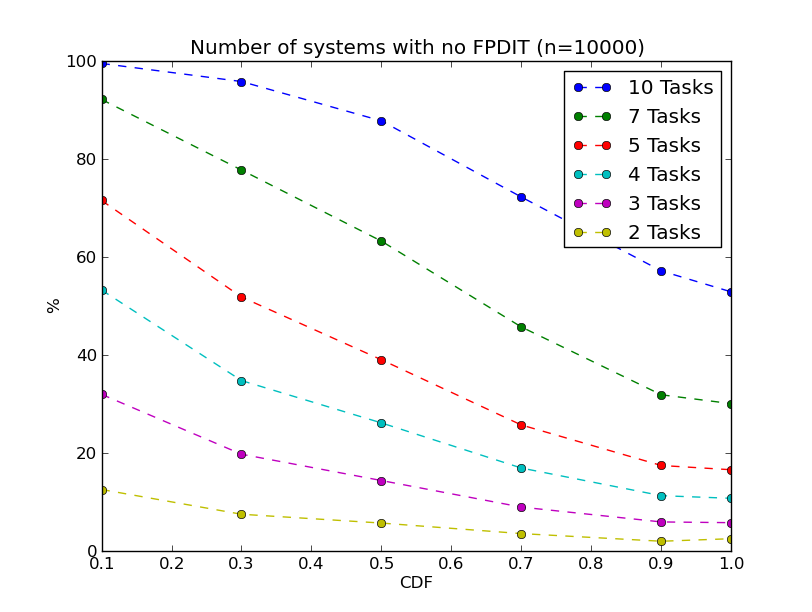
\includegraphics[width=0.4\textwidth]{figs/nofpdit_4.png}
	\end{center}
	\caption{Evolution of the existence of FPDIT with the CDF}
	\label{fig:noFPDIT}
	\end{figure}

	We observe that when the CDF is close to zero, fewer systems have a FPDIT.
	This is easily explained by the fact that
	a high CDF means more idle instants for each task, and thus more opportunities
	for DITs to happen. Similarly, as all tasks must be synchronized for a DIT to
	happen, a higher number of tasks results in a decrease in FPDIT density.

\section{C-space of asynchronous systems}
\label{sct:asyncCspace}

	\subsection{Description using DBF}

		The description based on \cite{baruah1999generalized} and presented in Section \ref{sct:cspaceDescr} was general and
		is still relevant. Therefore the C-space is still accurately described by
		the following infinite number of constraints:
		\begin{equation}
			\sum_{i=1}^{n} n_i(t_1, t_2)
			\, C_i \leq t_2 - t_1 \; \forall \: 0 \leq t_1 \leq t_2
		\end{equation}
		However, the method used in the synchronous case to remove redundancy does not
		apply here. A more general approach is presented in the following section.

	\subsection{Removing redundant constraints}

		The first two following sections contain well-known results of feasibility analysis.
		The third one is a new result based on the FPDIT and the last section contains a general
		but heavy method for removing constraints redundancies.

		\subsubsection{Job arrival and deadline}
			Consider a time interval $[t_1, t_2]$. If $t_2$ is an instant without any
			job deadline, then by definition the value of $\dbf{t_1, t_2}$ will be equal to
			$\dbf{t_1, t_2^*}$, where $t_2^*$ is the latest deadline before $t_2$.

			A similar argument can be made if $t_1$ is an instant without any job arrival
			(and $t_1^*$ is the earliest arrival after $t_1$). We can thus restrict
			ourselves to intervals where $t_1$ is an instant with at least one job
			arrival, and $t_2$ is an instant with at least one job deadline.

		\subsubsection{Feasibility interval}
			First let us recall how an asynchronous system behaves under an optimal
			scheduler, for example EDF.

			As shown in Fig. \ref{fig:asyncBehavior}, the system begins in the
			\emph{incomplete period}, where all tasks are not in the system. Then, after
			$O_{max}$ time units, every tasks is in the system and the \emph{transient
			period} begins. Then, after $O_{max} + H$ time units, the system is faced
			with the same pattern of arrival as in $O_{max}$. However, because in
			$O_{max} + H$ every task is in the system and in $O_{max}$ some were missing,
			the state of the system will be different. The \emph{stationary period} then
			begins. At instant $O_{max} + 2H$ it is guaranteed that the system is in the
			exact same situation it was at instant $O_{max} + H$.

			\begin{figure}[h]
				\[
					\begin{array}{r||c|c|c|l}
									& \text{Incomplete} & \text{Transient}	& \text{Stationary} & \cdots \\
						\text{Name} & \text{period} 	& \text{period} 	& \text{period}  	& \\ \hline
						\text{size} & O_{max} 			& H 				& H 				& \cdots \\ \hline
						t \geqslant & 0 				& O_{max} 			& O_{max} + H 		& \cdots
					\end{array}
				\]
				\begin{center}
				\caption{Behavior of an asynchronous system under EDF.}
				\label{fig:asyncBehavior}
				\end{center}
			\end{figure}

			For this reason, as shown by \cite{leung1982complexity}, it is sufficient (but pessimistic) to
			check for
			intervals included in the interval $[O_{max}, O_{max} + 2H]$, which has an exponential length
			in the number of tasks. A better interval is given in \cite{choquet2004minimal} using the
			notion of cyclic idle times (denoted $t_c$), which are dependent of the execution
			time and therefore cannot be used directly to characterize the C-Space. Their interval is $[0, t_c + H]$ and is valid for
			every cyclic idle time $t_c$.

			In the following section, we extend the latter interval using the previously defined notion
			of periodic DIT, a particular case of cyclic idle times which does not depend on the execution
			times.

\subsubsection{Using the first periodic DIT}

The FPDIT, if it exists, must occur in the transient period. Indeed, it cannot occur in the incomplete period by definition ($t_d > O_{max}$) and if it occurred in the $k^{th}$ stationary period, another DIT should have occurred in the transient period at instant $t_d - k H$ (a contradiction).

As the FPDIT happens when all tasks are in the system, we know that the system will arrive in the exact same state one hyperperiod later ($t_d + H$) (A rigorous proof is given in \cite{choquet2004minimal} for any cyclic idle time). We can thus restrict the DBF test to intervals included in the interval $[t_d, t_d + H]$ if the FPDIT exists. This will always be a better interval than $[O_{max}, O_{max} + 2H]$ and if the first periodic DIT does not exist (which can be verified as explained in Section \ref{sct:FPDITexist}), the latter interval can be used.

\subsubsection{Redundancy as an integer linear problem}

Previous sections give us a list of (integer) linear constraints accurately describing the C-space, composed of the DBF test applied to the required intervals. We now give a method to remove redundant constraints from this list.

The general problem of redundancy of some linear constraint $C \cdot X \leq d$
w.r.t. a set of previous linear constraints $A \cdot X \leq B$ in an ILP can
itself be written as the ILP presented in Fig.~\ref{fig:redILP}.

\begin{figure}[h]
$$z = \max C \cdot X$$
s.t.
\[
\begin{array}{rcc}
  A \cdot X &\leq & B \\
  C \cdot X &\leq & d + 1
\end{array}
%\begin{array}{rccc}
%  A & X &\leq & B \\
%  C & X &\leq & d + 1
%\end{array}
\]
with
\[
  \begin{array}{ccc}
    A & : & [n,k] \text{ matrix}\\
    B & : & [n,1] \text{ matrix}\\
    C & : & [n,1] \text{ matrix}\\
    X & : & [1,n] \text{ matrix}\\
    d & : & \text{integer}
  \end{array}
\]
\caption{Redundancy of $C \cdot X \leq d$ w.r.t. $A \cdot X \leq B$ as an ILP}
\label{fig:redILP}
\end{figure}

Indeed, if the maximization returns $z=d+1$, it means that there are some integer values accessible with the previous constraints that the new constraint forbids. On the other hands, if the maximization returns $z \leq d$, it means that the limitation expressed in the new constraint is already enforced by the previous constraints. Therefore $z \leq d$ is a necessary and sufficient condition of redundancy of the new constraint.

Such a linear problem can be solved by a branch-and-bound approach \cite{nemhauser1988integer}. However, in our case the problem is not to test for redundancy of a particular constraint but to find all redundant constraints within a set. A naive algorithm would consist of testing every constraint against all others. We present Algorithm \ref{alg:prunRedun}, which has the same theoretical complexity but is more efficient when most of the constraints are redundant. Indeed, most of the system we generated had a final C-space description size of less than five constraints, even if the initial description often contained more than a thousand.

\begin{algorithm}
\caption{Removing redundancy from CSPACE}
\label{alg:prunRedun}
  \begin{algorithmic}[1]
    \STATE $CSPACE$ : set of constraints
    \STATE $S \leftarrow \emptyset$
    \STATE \COMMENT{$1^{st}$ pass: test each $cstr$ against previous ones}
    \FOR{$cstr$ \textbf{in} $CSPACE$}
      \IF {$cstr$ is not redundant w.r.t. $S$}
        \STATE $S.push(cst)rcl$
      \ENDIF
    \ENDFOR
    \STATE \COMMENT{$2^{nd}$ pass: test remaining $cstr$ against every other}
    \FOR{$cstr$ \textbf{in} $S$}
      \STATE $cstr$ = $S.pop()$
      \IF {$cstr$ is not redundant w.r.t. $S$}
        \STATE $S.push(cstr)$
      \ENDIF
    \ENDFOR
    \RETURN{S}
  \end{algorithmic}
\end{algorithm}

This algorithm
has an exponential complexity in the number of constraints. The initial description
of the C-space should thus be as concise as possible.

To summarize, we first reduced the number of constraints from every possible
interval $[t_1, t_2]$ to the intervals where $t_1$ is an arrival time and
$t_2$ is a deadline in $[t_d, t_d + H]$ if $t_d$ exists, or in
$[O_{max}, O_{max} + 2H]$ otherwise. This set of constraints is a
correct but redundant description of the C-Space. Redundant
constraints are removed through a linear integer approach.

\section{Numerical Example}

Consider the following task system

    \begin{center}
    \begin{tabular}{|r|c|c|c|c|}
     \hline
      & $O_i$ & $C_i$ & $D_i$ & $T_i$ \\
     \hline
     $\tau_1$ & 8 & $C_1$ & 7 & 15\\
     \hline
     $\tau_2$ & 0 & $C_2$ & 2 & 5\\
     \hline
    \end{tabular}
    \end{center}

The FPDIT happens at $t=15$ and we have $H = 15$. The study interval using the FPDIT is thus $[15, 30]$, which contains 11 intervals $[a,d]$ with $a$ being the arrival of a job, $d$ being the deadline of a job, and $15 \leqslant a < d \leqslant 30$. Those intervals are
$[15, 17]$, $[15, 22]$, $[15, 27]$, $[15, 30]$, $[20, 22]$, $[20, 27]$, $[20, 30]$, $[23, 27]$, $[23, 30]$, $[25, 27]$ and $[25, 30]$. For comparison, the original study interval of $[O_{max}, O_{max} + 2H]$ is $[8, 38]$ which yields 57 intervals.

For each $[a, d]$, we have a constraint $$\sum_{i=1}^{n} n_i(a, d) \, C_i \leqslant d - a$$ which give a description of the C-space.

We now apply Algorithm \ref{alg:prunRedun} to remove redundancies, leaving us with the following constraints:
	\begin{equation}
		\left\{
			\begin{array}{ccccc}
				& & C_2 & \leqslant & 2 \\
				C_1 & + & C_2 & \leqslant & 7
			\end{array}
		\right.
	\end{equation}
The C-space thus contains 11 points $(C_1, C_2) = (1, 1)$, $(2, 1)$, $(3, 1)$, $(4, 1)$, $(5, 1)$, $(6, 1)$, $(1, 2)$, $(2, 2)$, $(3, 2)$, $(4, 2)$ and $(5, 2)$.

Let us now consider the same system but with a synchronous pattern of arrival ($O_1 = O_2 = 0$). The first DIT happens at time $t_d = 7$. The intervals to consider are thus of the form $[0, t]$ where $t$ is a deadline happening before or at time $t_d$. This yields two intervals ($[0, 2]$ and $[0, 7]$) and the following constraints describing the C-space, none of them being redundant:
$$
\left\{
  \begin{array}{ccccc}
    & & C_2 & \leqslant & 2 \\
    C_1 & + & 2 C_2 & \leqslant & 7
  \end{array}
\right.
$$
This time, the C-space only contains 8 points: $(1, 1)$, $(2, 1)$, $(3, 1)$, $(4, 1)$, $(5, 1)$, $(1, 2)$, $(2, 2)$, $(3, 2)$.

Fig. \ref{fig:cspaceComp} shows the two C-spaces in the plane. The dark gray region is the C-space of the synchronous system and the light gray region is the surface gain given by the asynchronous system.

\begin{figure}[h]
\begin{center}
  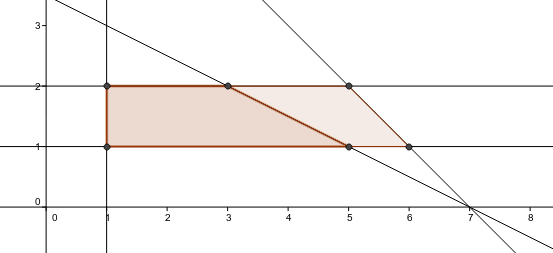
\includegraphics[width=0.3\textwidth]{figs/cspace_example.png}
  \caption{C-space of an asynchronous system and its corresponding synchronous system}
  \label{fig:cspaceComp}
\end{center}
\end{figure}


\section{Experimental C-space size gain of asynchronous systems}
\label{sct:expCspaceGain}
	One of the advantages of asynchronous systems over synchronous systems in the
	context of periodic tasks is that the critical instants of asynchronous systems
	can be less constraining for the C-space than synchronous instants (if offsets are chosen to prevent synchronous releases). For this reason, modifying task offsets when possible during
	the design of a real-time system is a useful trick to fit a heavy periodic task set
	into a given platform.

	In Fig.~\ref{fig:sizeRatio} a number of feasible asynchronous task sets of
	three tasks without synchronous instants were generated as described in Section~\ref{sct:noFPDITsimu}. The size of their
	C-space (number of valid WCET vectors) was compared with that of the same
	task sets with all offsets set to zero. The systems were generated as in section~\ref{sct:noFPDITsimu}
	and the integer linear problems used to remove redundancies were solved via the GLPK tool\footnote{\url{http://www.gnu.org/software/glpk/}}.

	In other words, fig.~\ref{fig:sizeRatio}
	evaluates the feasibility gain of adding random offsets w.r.t. a synchronous task
	set. Offsets eventually leading to synchronous releases have been discarded. The problem of offset assignment has been considered for example in \cite{grenier2008pushing} in the case of fixed WCET values. To the best of our knowledge, finding offsets maximizing a C-space region is an open problem.

	\begin{figure}[h]
		\begin{center}
			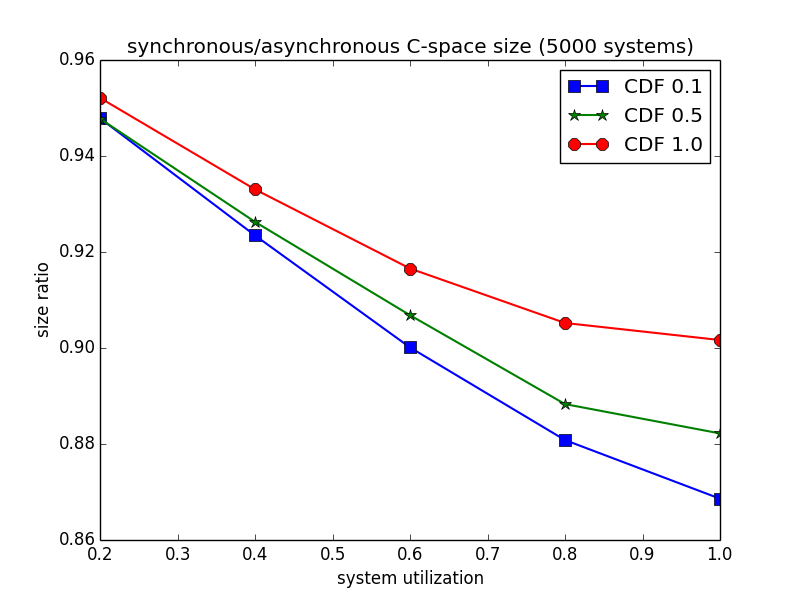
\includegraphics[width=0.4\textwidth]{figs/sizeratio.png}
			\caption{C-space size ratio between asynchronous and equivalent synchronous
			systems}
			\label{fig:sizeRatio}
		\end{center}
	\end{figure}

	The ratio between the size of the synchronous and asynchronous C-spaces of
	these systems roughly range from 0.95 in the worst case (high utilization, high
	CDF) to 0.85 in the best case (low utilization, low CDF). Each point on the graph is an average over 5000 tests.
	Note that the value of the CDF has a greater influence on this ratio than
	the system's total utilization, but less so when the CDF is higher. It is also
	important to note that even though a 0.95 ratio may not seem much, the
	synchronous C-spaces of the systems contain many dominated WCET vectors, and
	only those that are in the border (i.e. non-dominated) actually matter to the
	designer of the system. Using the asynchronous C-space instead will relax some
	constraints and therefore add new acceptable and dominating solutions,
	increasing the quality of the C-space border.

\section{Conclusion}

In this paper, we presented a general approach to concisely define the C-space of a constrained periodic task set for EDF on uniform platforms. We then used the C-space to quantify the feasibility gain given by random offset values, with a final result of about 10~\% more WCET values being feasible. Possible future works includes an extension to the study of systems with preemption costs or running on multiprocessor platforms, as the value of the DIT does not depend on preemptions or the number of processors.

Future works could also repeat the simulation of section~\ref{sct:expCspaceGain} with the algorithm described in \cite{grenier2008pushing}, which determine offset values with optimal feasibility for given WCET values. We could like to study if those heuristics obtained for particular WCETs scenarios can also be interesting for any WCET in the \mbox{C-Space}.

% Future works could also study the case of offset-free systems, where the offset values can be chosen. The performance of algorithms such as \cite{grenier2008pushing} and \cite{goossens2003scheduling} (although the latter depends on the execution times), which determine offset values with optimal feasibility, can be expressed using the C-space.

Another direction is to study the shape of the C-space and how it is affected by some factors. An
interesting path would be the effect of the CDF on the number of constraints describing the C-space,
as we know that in the implicit case this description is simple ($U_{tot} \leqslant 1$). While we
quantified the feasibility gain by looking at the ratio between sizes of C-space, another approach
would be to look at the ratio between the minimal distance of the border of the C-space, which would
give a lower bound of the gain given by the offsets.

% conference papers do not normally have an appendix


% use section* for acknowledgement
% \section*{Acknowledgment}


% The authors would like to thank...


% trigger a \newpage just before the given reference
% number - used to balance the columns on the last page
% adjust value as needed - may need to be readjusted if
% the document is modified later
%\IEEEtriggeratref{8}
% The "triggered" command can be changed if desired:
%\IEEEtriggercmd{\enlargethispage{-5in}}

% references section

% can use a bibliography generated by BibTeX as a .bbl file
% BibTeX documentation can be easily obtained at:
% http://www.ctan.org/tex-archive/biblio/bibtex/contrib/doc/
% The IEEEtran BibTeX style support page is at:
% http://www.michaelshell.org/tex/ieeetran/bibtex/
%\bibliographystyle{IEEEtran}
% argument is your BibTeX string definitions and bibliography database(s)
%\bibliography{IEEEabrv,../bib/paper}
%
% <OR> manually copy in the resultant .bbl file
% set second argument of \begin to the number of references
% (used to reserve space for the reference number labels box)
% \nocite{*}
\bibliographystyle{IEEEtran}
\bibliography{dit-paper}


% that's all folks
\end{document}


